\subsection{Lasso Regression}

Our last method is the Lasso Regression. In figure \Fig~\ref{fig:LassoCoefVsLambda} are shown the coefficients' behavior as $\lambda$ increases. 

\begin{figure}[h]
	\centering
	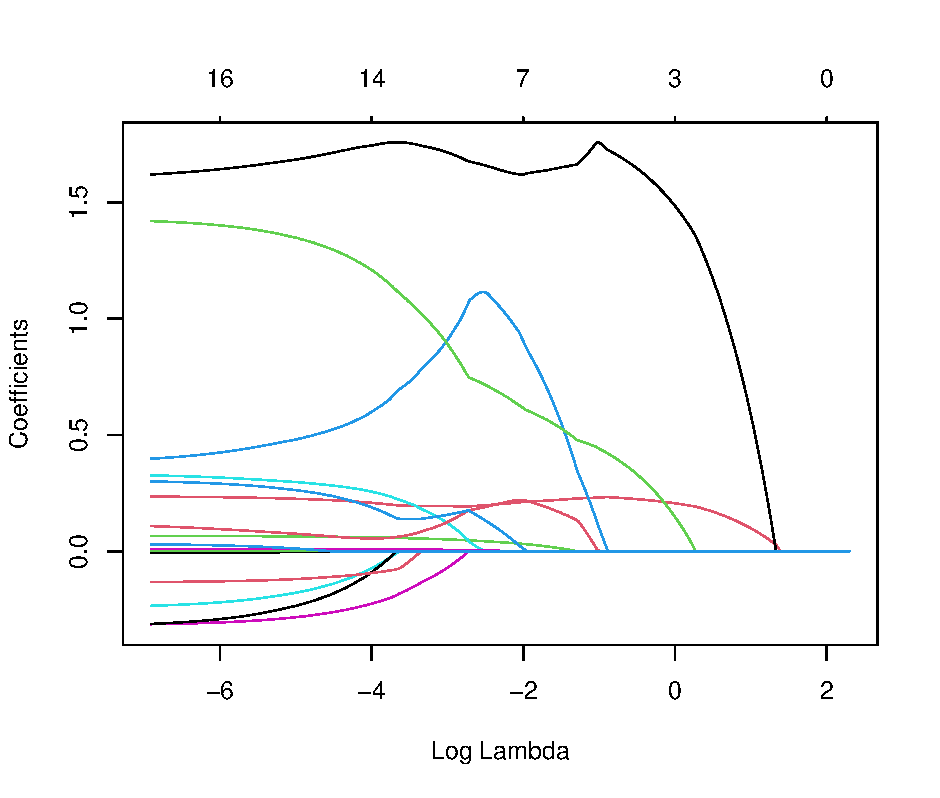
\includegraphics[width=0.5\linewidth]{ImageFiles/Regression/Lasso/LassoCoefVsLambda}
	\caption{The ridge regression coefficients as function of $\lambda$.}
	\label{fig:LassoCoefVsLambda}
\end{figure}

The same procedure applied for the Ridge is followed again. In figure \Fig~\ref{fig:LassoCvPlot} is possible the trend of the cross validated MSE("\textit{Mean Square Error}") when $\lambda$ increases. The optimal value was found to be $\lambda_{opt} = 0$, that means to penalization. The result is coherent with what obtained from Ridge Regression. Penalization in our case is not helpful.

\begin{figure}[h]
	\centering
	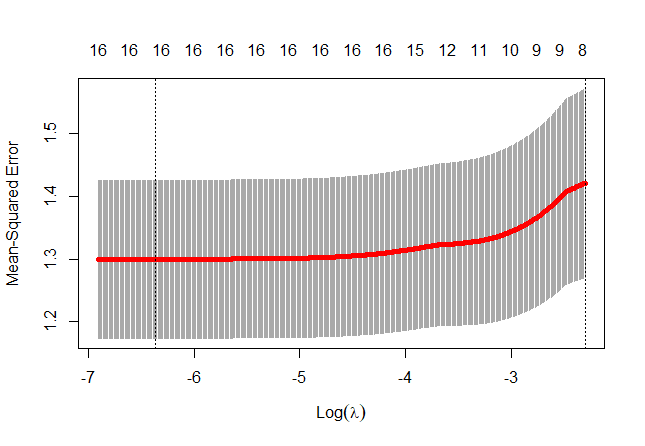
\includegraphics[width=0.7\linewidth]{ImageFiles/Regression/Lasso/LassoCvPlot}
	\caption{The Cross Validated MSE as function of $\lambda$.}
	\label{fig:LassoCvPlot}
\end{figure}